\documentclass[aps,pra,twocolumn,reprint,amsmath,amssymb]{revtex4-2}

\usepackage{graphicx}
\usepackage{booktabs}
\usepackage{siunitx}
\usepackage[colorlinks=true,linkcolor=blue,citecolor=blue,urlcolor=blue]{hyperref}
\usepackage{float}
\usepackage{xcolor}
\usepackage{braket}

\begin{document}

\title{Cluster-State Unitary Decomposition with Native Free Evolution and SNAP}
\author{Codex}
\affiliation{Quantum Circuits Group}
\date{\today}

\begin{abstract}
We study how much of the cluster-state transfer unitary in a dispersive
transmon-cavity system can be implemented by native free evolution alone, and
how that answer changes once photon-number selective phase gates (SNAP) are
added. The logical target acts on
$\{\ket{g,0},\ket{g,1},\ket{e,0},\ket{e,1}\}$ and is
$U_{\mathrm{cl}}=\mathrm{SWAP}\cdot\mathrm{CZ}\cdot(H\otimes I)$. The baseline
gate set is restricted to displacement, qubit rotations, and a wait-only
entangling primitive with optimized duration. Extended families add SNAP either
as a final correction layer, interleaved after each free-evolution block, or in
both roles. Using \texttt{cqed\_sim} for all synthesis and diagnostics, we find
that native free evolution is indispensable: removing it from the best native
sequence drops the logical fidelity to 0.167, and removing it from the best
SNAP-assisted sequence drops the fidelity to 0.322. SNAP is therefore not a
replacement entangler. It is also not purely redundant. The best no-SNAP family
reaches fidelity 0.964 with six free-evolution blocks, depth 20, and total wait
time \SI{1018}{ns}. The best SNAP-extended family reaches 0.988 with six
free-evolution blocks and six interleaved SNAP layers at essentially the same
wait budget (\SI{1027}{ns}), indicating that SNAP mainly supplies explicit
cavity-only phase correction rather than reducing the native entangling load at
the highest-fidelity point. At a practical threshold of 0.95 fidelity, however,
SNAP reduces the required entangling resources: the interleaved family reaches
0.964 with four free-evolution blocks, depth 18, and \SI{769}{ns} total wait
time, whereas the no-SNAP family first exceeds 0.95 only at six blocks, depth
20, and \SI{1018}{ns}. A follow-up improvement pass then re-optimizes the two
depth-6 winners at $N_{\mathrm{cav}}=6$, raising the native case from replay
fidelity 0.9177 to 0.9234 and the interleaved-SNAP case from 0.9473 to 0.9908.
Coherent model-backed replay at $N_{\mathrm{cav}}=8$ gives 0.9238 and 0.9867,
while a documented Lindblad noise surrogate yields mean probe-state fidelities
0.8907 and 0.9351, respectively. Tail-only SNAP layers provide little benefit.
\end{abstract}

\maketitle

\section{Introduction}
Cluster-state generation by repeated application of a fixed transfer unitary is
a standard route to measurement-based quantum computation
\cite{raussendorf2001one}. In circuit QED, the natural hardware platform is a
dispersively coupled qubit-oscillator pair, where native dispersive waiting,
cavity displacements, qubit rotations, and oscillator phase gates all provide
different pieces of the required control toolbox \cite{blais2021circuit,
heeres2015snap,krastanov2015universal,eickbusch2022ecd}. The key design
question here is narrower than full universality: when the target is the
four-dimensional cluster-state transfer unitary, which part of the job is done
by native free evolution and which part genuinely benefits from explicit
number-dependent phase programming?

Earlier work in this repository established that the cluster target can be
implemented either by broader selective gate libraries or by direct optimal
control, but that result did not isolate the role of the wait-only entangler.
The present study does. We first restrict the search to
$\{D,R_q,U_{\mathrm{FE}}(t)\}$, where $U_{\mathrm{FE}}(t)$ is a no-drive
free-evolution conditional-phase gate with optimized wait time. We then compare
against extended families that add SNAP layers in different positions. This lets
us answer three concrete questions: does SNAP reduce gate depth, does it reduce
the total entangling wait time needed for useful fidelities, and does it add
independent functionality or mostly redundant phase freedom?

\section{System and Methods}
\subsection{Hamiltonian}
We use the dispersive transmon-cavity model already implemented in
\texttt{cqed\_sim} \cite{cqedsim}. In the rotating frame used by the synthesis
stack,
\begin{equation}
\frac{H}{\hbar} =
\omega_c a^\dagger a + \omega_q b^\dagger b
+ \frac{\alpha}{2} b^{\dagger 2} b^2
+ \chi\, a^\dagger a\, b^\dagger b
+ \chi' a^{\dagger 2} a^2 b^\dagger b
+ \frac{K}{2} a^{\dagger 2} a^2 ,
\end{equation}
with $a$ the cavity annihilation operator, $b$ the transmon lowering operator,
$\chi$ the dispersive shift, $\chi'$ the first higher-order dispersive
correction, and $K$ the cavity self-Kerr. The logical basis is
\begin{equation}
\mathcal{B}_{\mathrm{log}} =
\{\ket{g,0},\ket{g,1},\ket{e,0},\ket{e,1}\},
\end{equation}
and the target unitary is
\begin{equation}
U_{\mathrm{cl}} = \mathrm{SWAP}\cdot\mathrm{CZ}\cdot(H\otimes I),
\end{equation}
equivalently \texttt{make\_target("cluster", n\_match=1)}.

\subsection{Simulation Parameters}
\begin{table}[H]
  \centering
  \caption{System and nominal gate parameters used in the decomposition study.}
  \begin{tabular}{@{}lll@{}}
    \toprule
    Parameter & Value & Unit \\
    \midrule
    $\omega_q / 2\pi$ & 6.150 & GHz \\
    $\omega_c / 2\pi$ & 5.241 & GHz \\
    $\alpha / 2\pi$ & -255 & MHz \\
    $\chi / 2\pi$ & -2.84 & MHz \\
    $\chi' / 2\pi$ & -21 & kHz \\
    $K / 2\pi$ & -28 & kHz \\
    $N_{\mathrm{tr}}$ & 2 & levels \\
    $N_{\mathrm{cav}}$ (search) & 4 & Fock states \\
    $D(\alpha)$ duration & 80 & ns \\
    $R_q(\theta,\phi)$ duration & 40 & ns \\
    SNAP duration & 200 & ns \\
    FE wait bounds & 40--400 & ns \\
    \bottomrule
  \end{tabular}
\end{table}

\subsection{Computational Approach}
All searches use the \texttt{cqed\_sim.unitary\_synthesis} stack
\cite{cqedsim}: \texttt{Displacement}, \texttt{QubitRotation},
\texttt{FreeEvolveCondPhase}, \texttt{SNAP}, \texttt{GateSequence},
\texttt{TargetUnitary}, \texttt{Subspace}, and \texttt{UnitarySynthesizer}.
The optimization objective combines unitary fidelity and leakage penalty, with a
small duration-weight sweep used only for compactness diagnostics. We use a
two-stage workflow: a coarse screening pass with 20 iterations and seed 17,
followed by refinement of the best case in each family with 35 iterations and
seeds 17 and 42.

Four families were searched:
\begin{align}
\mathcal{G}_{\mathrm{FE}} &: [D\,R\,\mathrm{FE}]^b D R, \\
\mathcal{G}_{\mathrm{tail}} &: [D\,R\,\mathrm{FE}]^b D\,\mathrm{SNAP}\,R, \\
\mathcal{G}_{\mathrm{int}} &: [D\,R\,\mathrm{FE}\,\mathrm{SNAP}]^b D R, \\
\mathcal{G}_{\mathrm{hyb}} &: [D\,R\,\mathrm{FE}\,\mathrm{SNAP}]^b D\,\mathrm{SNAP}\,R.
\end{align}
Here $b$ is the number of free-evolution blocks. The baseline family
$\mathcal{G}_{\mathrm{FE}}$ isolates the native wait-only entangler. The other
families test whether SNAP is useful as a final clean-up layer, as an
interleaved correction after each entangling wait, or in both roles.

To attribute phase generation, we use two diagnostics already exposed by
\texttt{cqed\_sim}: \texttt{GateSequence.phase\_decomposition(...)} for
per-gate drift and SNAP phase tables, and
\texttt{logical\_block\_phase\_diagnostics(...)} to compare strict logical
fidelity against a cavity-block gauge. Complexity is quantified by gate depth,
parameter count, SNAP gate count, SNAP phase count, and total free-evolution
wait time.

\section{Results}
\subsection{No-SNAP Free-Evolution Baseline}
Figure~\ref{fig:depth} shows the fidelity-depth landscape across all screened
families. The no-SNAP baseline improves steadily but slowly as additional
free-evolution blocks are added. Its best refined case is
\texttt{native\_fe\_b6}, which reaches fidelity 0.9639 with gate depth 20,
total sequence duration \SI{1858}{ns}, and total entangling wait time
\SI{1018}{ns}. The corresponding complexity counts are 48 continuous parameters
and six entangling waits, with no explicit phase gates.

\begin{figure}[H]
  \centering
  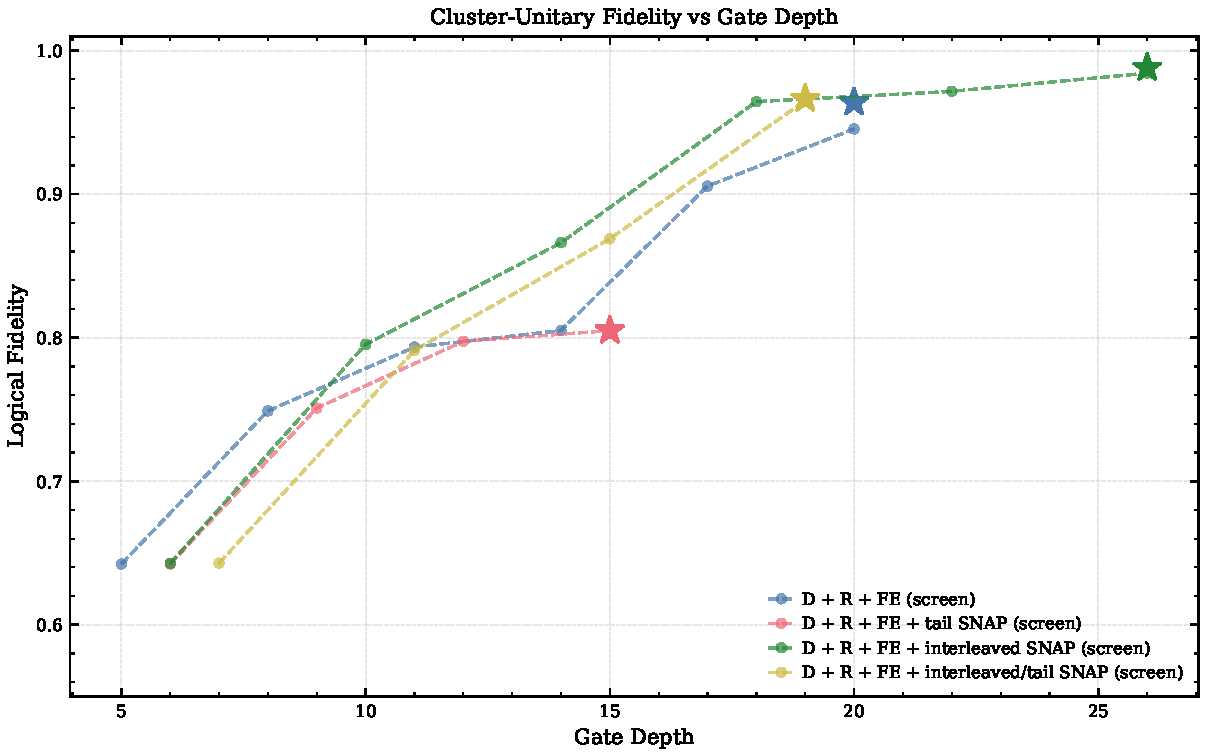
\includegraphics[width=\linewidth]{../figures/fidelity_vs_depth.pdf}
  \caption{Logical fidelity versus gate depth for the screened and refined
  families. The stars denote the best refined case in each family. Interleaved
  SNAP layers improve the achievable fidelity but do not dominate the pure
  native family at low depth.}
  \label{fig:depth}
\end{figure}

The ablation data in Table~\ref{tab:ablation} shows that free evolution is the
essential entangling resource. Removing every FE block from the best native
sequence drops the fidelity from 0.9639 to 0.1675, while the block-gauge
fidelity falls to 0.2640. This is consistent with the primitive definitions:
\texttt{Displacement} and \texttt{QubitRotation} provide mixing, but only
\texttt{FreeEvolveCondPhase} produces qubit-conditioned phases in the restricted
no-SNAP family.

\subsection{SNAP-Extended Families}
The extended families separate cleanly into one ineffective and two useful
patterns. Tail-only SNAP layers are almost useless: the best refined
\texttt{snap\_tail\_b4} case reaches only 0.8050, essentially matching the
native four-block result. This means a single cavity-only phase layer added at
the end cannot rescue a poor free-evolution decomposition.

Interleaved SNAP layers are different. The best refined
\texttt{snap\_interleaved\_b6} case reaches 0.9881 with six FE blocks and six
SNAP layers, compared with 0.9639 for the best native six-block sequence. The
total entangling wait time is almost unchanged: \SI{1027}{ns} versus
\SI{1018}{ns}. The price is complexity: gate depth rises from 20 to 26, the
parameter count rises from 48 to 78, and the sequence now contains 24 explicit
SNAP phase parameters. Interleaved SNAP therefore improves fidelity mainly by
adding cavity-only correction freedom, not by replacing the entangler.

The hybrid family, which adds one extra tail SNAP on top of the interleaved
structure, reaches 0.9665 with four FE blocks and five SNAPs. This is useful as
a moderate-depth compromise, but it does not beat the best interleaved sequence
in fidelity. The additional tail SNAP is therefore not the decisive ingredient.

\begin{figure}[H]
  \centering
  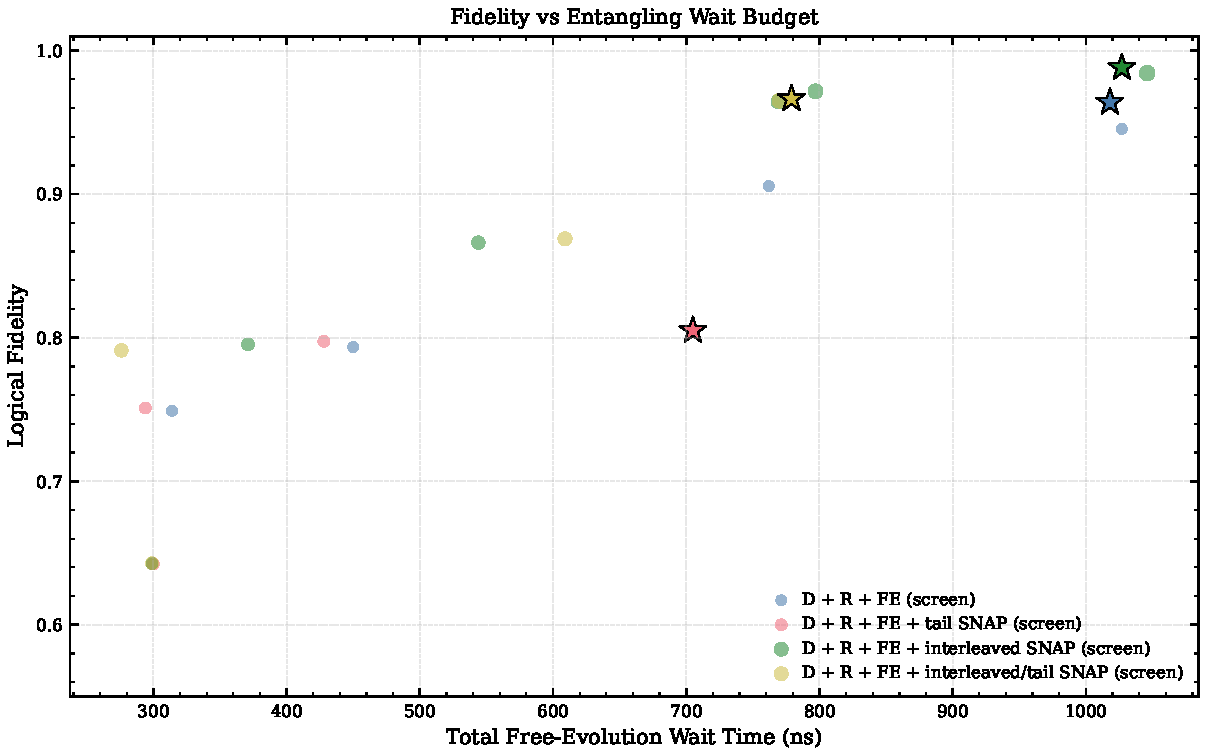
\includegraphics[width=\linewidth]{../figures/wait_vs_fidelity.pdf}
  \caption{Logical fidelity versus total free-evolution wait time. The
  high-fidelity region is entered by SNAP-assisted families at smaller wait
  budgets than the no-SNAP baseline, but the absolute best-fidelity point still
  uses roughly the same total wait time as the best native sequence.}
  \label{fig:wait}
\end{figure}

\subsection{Does SNAP Reduce Depth, Wait Time, or Only Add Redundancy?}
The answer depends on which comparison point is used.

At the absolute best-fidelity endpoint, SNAP does \emph{not} reduce the total
wait time or depth. The best native and best interleaved cases both use six FE
blocks and about \SI{1.02}{\micro\second} of total waiting, while the
SNAP-assisted sequence is deeper and more parameter-rich. In that sense SNAP is
not a shortcut entangler.

At practical fidelity thresholds, however, SNAP is clearly helpful. The first
native case above 0.95 fidelity is \texttt{native\_fe\_b6}, with depth 20 and
\SI{1018}{ns} of waiting. By contrast, the interleaved SNAP family already
reaches 0.9644 at \texttt{snap\_interleaved\_b4}, with depth 18 and only
\SI{769}{ns} of waiting. Relative to the no-SNAP threshold case, this is a
24.5\% reduction in total entangling wait time and a reduction of two gates in
depth. The same family reaches 0.9716 with five FE blocks and \SI{797}{ns}
wait, while the no-SNAP family never crosses 0.97 in the screened-plus-refined
set.

Phase-budget and ablation data clarify the mechanism. The best native and best
SNAP-assisted sequences accumulate nearly identical logical FE phase budgets:
5.78$\pi$ and 5.83$\pi$, respectively. The best SNAP-assisted sequence adds an
extra 1.14$\pi$ of explicit logical cavity phase through its SNAP layers. When
all SNAPs are removed from that sequence, the fidelity drops from 0.9881 to
0.4850 even though the FE budget is unchanged. When all FE blocks are removed,
the fidelity falls further to 0.3223. Thus FE supplies the entangling phase,
while SNAP supplies additional cavity-only phase correction that is independent
and useful but not sufficient by itself.

\begin{figure}[H]
  \centering
  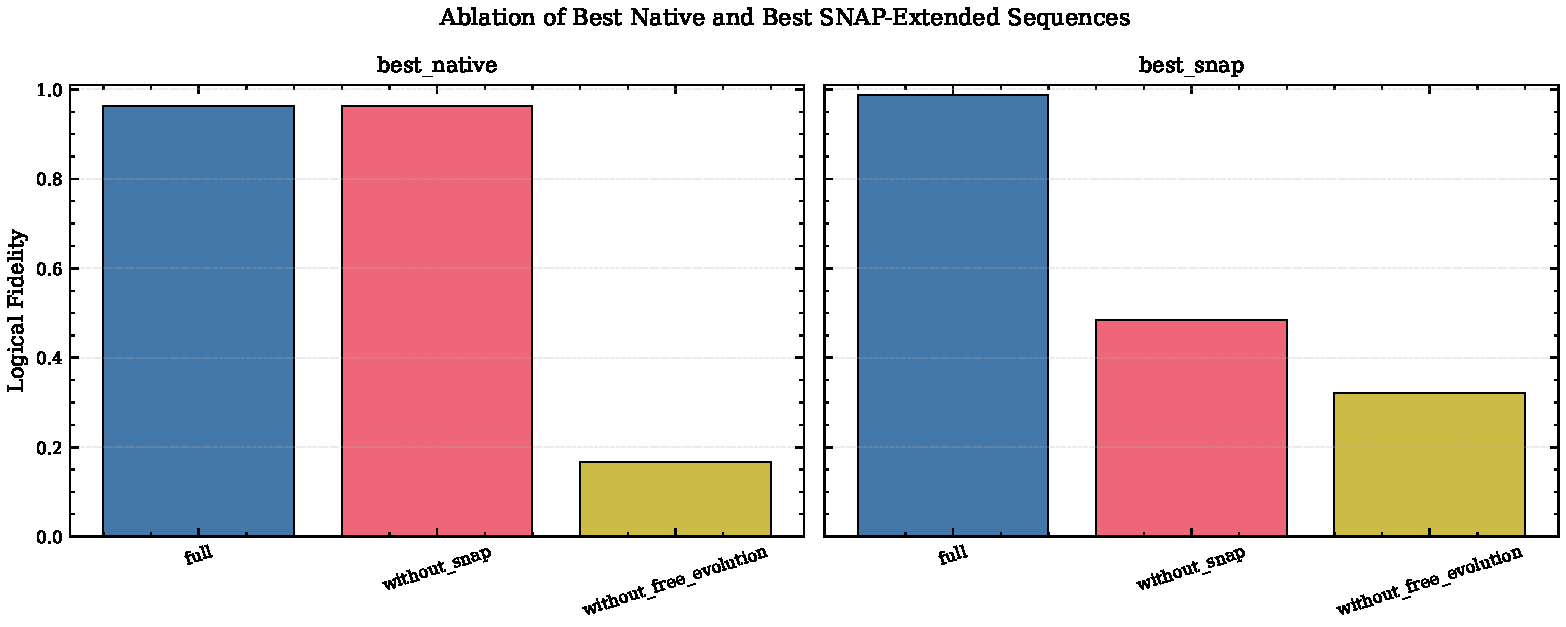
\includegraphics[width=\linewidth]{../figures/sequence_ablations.pdf}
  \caption{Ablation of the best native and best SNAP-assisted sequences.
  Removing free evolution destroys both constructions. Removing SNAP from the
  best SNAP-assisted sequence also destroys high fidelity, confirming that FE
  and SNAP play distinct roles rather than one replacing the other.}
  \label{fig:ablation}
\end{figure}

\begin{figure}[H]
  \centering
  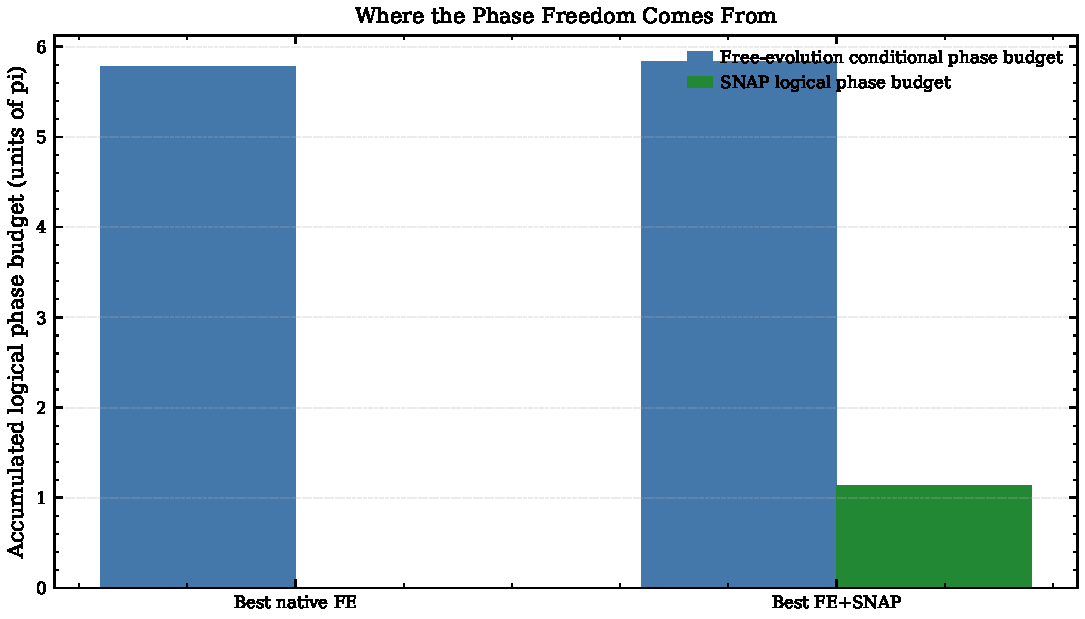
\includegraphics[width=\linewidth]{../figures/phase_budget_comparison.pdf}
  \caption{Phase-budget attribution for the best native and best SNAP-assisted
  sequences. Both use roughly the same amount of qubit-conditioned phase from
  free evolution; the SNAP-assisted solution adds an extra cavity-only phase
  budget of about 1.14$\pi$.}
  \label{fig:phasebudget}
\end{figure}

\begin{table}[H]
  \centering
  \caption{Best refined result from each family.}
  \label{tab:familybest}
  \begin{tabular}{@{}lccccc@{}}
    \toprule
    Family & $F$ & Depth & Wait (ns) & SNAPs & Params \\
    \midrule
    Native FE & 0.9639 & 20 & 1018 & 0 & 48 \\
    Tail SNAP & 0.8050 & 15 & 705 & 1 & 39 \\
    Interleaved SNAP & \textbf{0.9881} & 26 & 1027 & 6 & 78 \\
    Hybrid SNAP & 0.9665 & 19 & 779 & 5 & 59 \\
    \bottomrule
  \end{tabular}
\end{table}

\begin{table}[H]
  \centering
  \caption{Ablation fidelities for the best native and best SNAP-assisted
  sequences.}
  \label{tab:ablation}
  \begin{tabular}{@{}lccc@{}}
    \toprule
    Case & Full & Without SNAP & Without FE \\
    \midrule
    Best native FE & 0.9639 & 0.9639 & 0.1675 \\
    Best FE+SNAP & 0.9881 & 0.4850 & 0.3223 \\
    \bottomrule
  \end{tabular}
\end{table}

\section{Validation}
\subsection{Sanity Checks}
The ablation study is the main sanity check. In the native family, eliminating
FE destroys the decomposition, which matches the expectation that the no-SNAP
family has no other entangling primitive. In the SNAP-assisted family, removing
SNAP also destroys the decomposition, showing that the added explicit phase
freedom is doing nontrivial work and is not merely idle redundancy. The near
equality of strict and cavity-block-gauge fidelities for the best cases further
shows that the remaining errors are not dominated by a removable block phase.

\subsection{Convergence Analysis}
The original winning sequences were first replayed without re-optimization at
larger cavity truncation. The best native sequence dropped from 0.9639 at
$N_{\mathrm{cav}}=4$ to 0.9177 and 0.9188 at $N_{\mathrm{cav}}=6$ and 8. The
best SNAP-assisted sequence dropped from 0.9881 to 0.9473 and 0.9433 over the
same truncation sweep. A follow-up improvement pass then re-optimized the two
depth-6 winners directly at $N_{\mathrm{cav}}=6$. This lifted the native family
to 0.9234 and the interleaved-SNAP family to 0.9908 at the larger truncation.
When those re-optimized winners are replayed coherently with the
model-backed pulse-unitary backend at $N_{\mathrm{cav}}=8$, the fidelities are
0.9238 (native) and 0.9867 (interleaved SNAP). The ranking is therefore much
more stable than the original replay-only validation suggested, although the
larger-truncation search has still not been repeated for every family and block
count.

\subsection{Noise Surrogate}
The present \texttt{cqed\_sim} build does not provide a direct noisy compiled
replay for sequences containing \texttt{FreeEvolveCondPhase} and \texttt{SNAP}:
the waveform bridge rejects both gates, and the gate-sequence \texttt{pulse}
backend ignores \texttt{NoiseSpec} during state propagation. We therefore added
a documented Lindblad surrogate that uses each gate's full pulse-unitary matrix
and duration to construct a finite-duration effective Hamiltonian, then evolves
the probe states with nominal $T_1=\SI{30}{\micro\second}$,
$T_\phi=\SI{20}{\micro\second}$, and cavity $T_1=\SI{200}{\micro\second}$.
At $N_{\mathrm{cav}}=6$, the mean probe-state fidelity falls from 0.9190 to
0.8904 for the re-optimized native family and from 0.9910 to 0.9387 for the
re-optimized interleaved-SNAP family. At $N_{\mathrm{cav}}=8$, the same
surrogate gives 0.8907 and 0.9351, respectively, so the qualitative ordering
survives under the nominal coherence budget.

\begin{figure}[H]
  \centering
  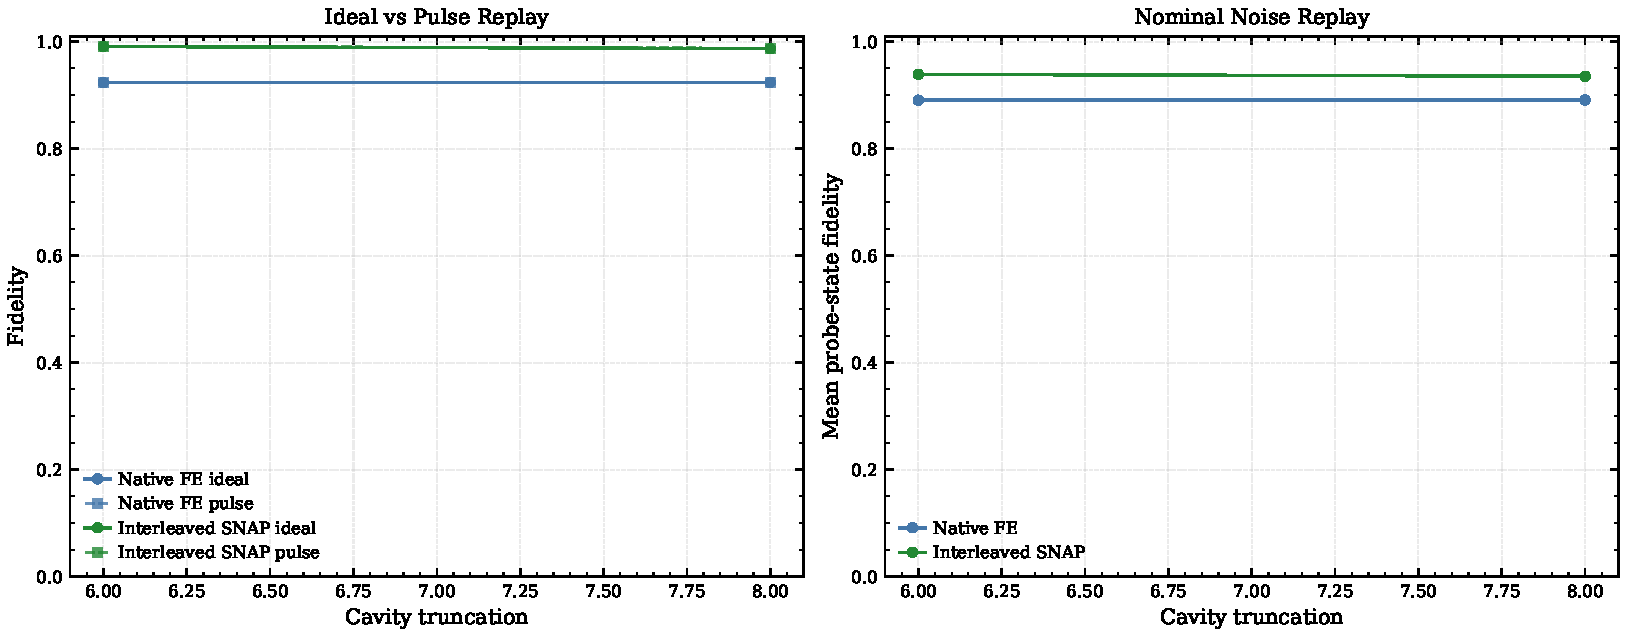
\includegraphics[width=\linewidth]{../figures/improvement_truncation_noise_summary.pdf}
  \caption{Improvement-pass validation. Left: ideal versus coherent pulse replay
  for the re-optimized depth-6 native and interleaved-SNAP winners at
  $N_{\mathrm{cav}}=6$ and 8. Right: nominal-noise Lindblad surrogate mean
  probe-state fidelity for the same two winners. The interleaved-SNAP sequence
  remains better at every tested truncation and under the nominal noise model.}
  \label{fig:trunc}
\end{figure}

\subsection{Reference Comparison}
There is no direct literature benchmark for this exact restricted gate-set
comparison. The observed hierarchy is nevertheless consistent with the general
bosonic-control literature: native waiting supplies the dispersive conditional
phase, while SNAP provides cavity-only phase programmability
\cite{heeres2015snap,krastanov2015universal}. Our best FE+SNAP sequence remains
below the stronger ideal-gate reference decompositions obtained previously in
this repository with broader selective gate libraries, which is expected because
the present study intentionally restricts the primitive set to isolate the role
of free evolution.

\section{Discussion}
The requested comparison yields a fairly nuanced answer. SNAP is not redundant,
because the best interleaved FE+SNAP sequence loses half of its fidelity if the
SNAP layers are removed while keeping the FE waits fixed. It is also not an
alternate entangler, because removing FE is even more destructive and because
the FE phase budget remains essentially unchanged between the best native and
best SNAP-assisted solutions. The cleanest interpretation is that native free
evolution carries the entangling burden and SNAP acts as an explicit local phase
compiler around that entangler.

This interpretation also explains why the best-fidelity endpoint does not use
less wait time with SNAP. To maximize fidelity, the optimizer still wants about
six FE blocks and about \SI{1}{\micro\second} of total waiting. What SNAP buys
is not a smaller FE phase budget, but the freedom to correct residual cavity
phases and leakage-inducing mismatches produced by the displacement-rotation-wait
structure. That is why the interleaved family crosses useful fidelity thresholds
earlier in depth, even though its absolute best solution is more complex than
the best native one.

The tail-only result is also informative. If SNAP were only needed as a final
phase clean-up, then one tail SNAP should have helped substantially. It did not.
The useful role of SNAP is therefore local and distributed: phase corrections
must be applied while the decomposition is being built, not only after it is
finished. By contrast, the extra tail SNAP in the hybrid family provides only a
small improvement over the four-block interleaved construction, which suggests
that much of the tail phase freedom is redundant once the interleaved layers are
already present.

The larger-truncation extension materially strengthens this interpretation.
Re-optimizing only the two depth-6 winners at $N_{\mathrm{cav}}=6$ already
changes the quantitative story: the native family improves only modestly, from
0.9177 to 0.9234, whereas the interleaved-SNAP family jumps from 0.9473 to
0.9908. In other words, the larger truncation does not simply punish the
SNAP-assisted sequence; it also reveals that the original $N_{\mathrm{cav}}=4$
parameter set left significant high-truncation performance on the table for the
interleaved construction.

The noise-surrogate extension points the same way. Under a shared nominal
coherence budget, the re-optimized interleaved-SNAP sequence still outperforms
the re-optimized native one by about 4.5 percentage points in mean probe-state
fidelity at both $N_{\mathrm{cav}}=6$ and 8. That does not settle the final
hardware story, because the noisy result is currently a documented surrogate
rather than a compiled cqed\_sim replay, but it does remove the most obvious
counter-argument that the deeper SNAP sequence must automatically lose once
decoherence is included.

\section{Conclusion}
The study goals were met. We isolated the native free-evolution family,
compared it against several SNAP-extended gate sets, identified which
contributions come from FE versus explicit phase gates, and quantified the trade
offs in fidelity, depth, wait time, and complexity.

The main conclusions are:
\begin{itemize}
  \item Native free evolution is essential. It is the only entangling resource
  in the restricted family, and removing it destroys the decomposition.
  \item SNAP is useful but not as a substitute entangler. Its benefit is to add
  cavity-only phase correction on top of essentially the same FE phase budget.
  \item At the best-fidelity endpoint, SNAP improves fidelity from 0.9639 to
  0.9881 but does not reduce the required total wait time; it increases depth
  and parameter count instead.
  \item At practical thresholds, SNAP reduces resource requirements. The
  interleaved family exceeds 0.95 fidelity with four FE blocks and
  \SI{769}{ns} of total wait, while the native family first exceeds 0.95 only
  with six FE blocks and \SI{1018}{ns} of wait.
  \item Tail-only SNAP is largely redundant, whereas interleaved SNAP is the
  meaningful extension.
  \item A larger-truncation improvement pass strengthens rather than weakens the
  SNAP conclusion: re-optimizing the two depth-6 winners at $N_{\mathrm{cav}}=6$
  yields 0.9234 for native FE and 0.9908 for interleaved SNAP, and the
  interleaved sequence remains ahead under both coherent replay and the nominal
  Lindblad noise surrogate.
\end{itemize}

\section{Limitations and Future Work}
\subsection{Known Limitations}
The first limitation is larger-truncation search coverage. The improvement pass
re-optimized only the two depth-6 winners at $N_{\mathrm{cav}}=6$; it did not
repeat the full family and block-count sweep at $N_{\mathrm{cav}}\geq 6$.
The updated numbers therefore establish that the native-vs-SNAP ranking
survives a stronger truncation and even sharpens in favor of interleaved SNAP,
but they do not yet prove that the original threshold frontiers remain globally
optimal at larger cutoff.

The second limitation is replay realism. Coherent replay now exists via the
model-backed pulse-unitary path, but the present \texttt{cqed\_sim} waveform
bridge still does not compile \texttt{FreeEvolveCondPhase} or \texttt{SNAP}
into hardware-distorted pulses. The current pulse-level result is therefore a
control surrogate, not a full compiled waveform validation.

The third limitation is noisy validation methodology. The direct gate-sequence
\texttt{pulse} backend ignores \texttt{NoiseSpec} during state propagation for
these FE/SNAP sequences, so the present decoherence analysis uses a documented
local Lindblad surrogate derived from the per-gate pulse-unitary matrices and
durations. This is more informative than a pure coherence-budget estimate, but
it remains a surrogate rather than a native compiled noisy replay.

The fourth limitation is optimization scope. We searched structured ansatz
families with modest multistart budgets, not an exhaustive global optimum. In
particular, a sparse-SNAP search that allows fewer than one SNAP per FE block at
high depth may find a lower-complexity solution than the present best
interleaved sequence.

\subsection{Suggested Improvements}
\begin{itemize}
  \item \textbf{[P1 | HIGH]} Repeat the full family/block-count search at
  $N_{\mathrm{cav}}\geq 6$ (and eventually $N_{\mathrm{cav}}=8$, $N_{\mathrm{tr}}=3$),
  rather than re-optimizing only the two depth-6 winners. The current extension
  confirms the ranking for those winners but does not yet establish the larger-
  truncation threshold frontier globally.
  \item \textbf{[P2 | HIGH]} Replace the local Lindblad surrogate with a direct
  compiled noisy replay. This requires either waveform-bridge support for
  \texttt{FreeEvolveCondPhase} and \texttt{SNAP} or a native noisy Hamiltonian-
  slice runner for gate sequences.
  \item \textbf{[P2 | MEDIUM]} Search sparse interleaved SNAP patterns at larger
  truncation. The best solution still uses six SNAP layers, but the tail-only
  family is ineffective and the hybrid tail layer appears weak, so some SNAP
  placements are probably redundant.
  \item \textbf{[P2 | LOW]} Add a wait-budget constrained search instead of only
  a duration-weight sweep. In the current fixed-depth frontier, the optimizer
  compressed non-wait gate durations much more than the FE budget.
  \item \textbf{[P3 | LOW]} Compare the best FE+SNAP sequence to broader
  selective references and to GRAPE warm starts to see whether the present
  restricted decomposition is a useful compiler seed.
\end{itemize}

\subsection{Open Questions}
The main open question is whether the best FE+SNAP sequence genuinely needs one
SNAP after every FE block, or whether a sparser pattern can retain most of the
fidelity gain. A second question is whether the observed threshold improvement
for SNAP persists after re-optimization at larger truncation. A third is whether
the same qualitative conclusion holds for larger logical subspaces or other
bosonic encodings, where the balance between native waiting and explicit phase
programming may shift.

\bibliographystyle{apsrev4-2}
\bibliography{references}

\appendix

\section{Detailed Results and Data}
Table~\ref{tab:familybest} gives the best refined result from each family. The
full screened landscape is stored in
\texttt{data/screen\_results.json}, and the refined winners are stored in
\texttt{data/refined\_results.json}. The most useful threshold-level comparison
is:
\begin{itemize}
  \item Native FE first exceeds 0.95 fidelity at \texttt{native\_fe\_b6}:
  depth 20, wait \SI{1018}{ns}, fidelity 0.9639.
  \item Interleaved FE+SNAP first exceeds 0.95 fidelity at
  \texttt{snap\_interleaved\_b4}: depth 18, wait \SI{769}{ns}, fidelity 0.9644.
  \item Interleaved FE+SNAP first exceeds 0.97 fidelity at
  \texttt{snap\_interleaved\_b5}: depth 22, wait \SI{797}{ns}, fidelity 0.9716.
\end{itemize}
These threshold points are saved in \texttt{data/threshold\_summary.json}.

\section{Reproducibility}
\subsection{Optimized Parameters}
The full optimized gate parameters are provided in machine-readable form in
\texttt{artifacts/best\_native\_sequence.json} and
\texttt{artifacts/best\_snap\_sequence.json}. Each artifact lists every gate in
order, including duration, optimized displacement amplitudes, qubit-rotation
angles/phases, FE wait times, and every SNAP phase.

\subsection{Waveform and Pulse Information}
This study used ideal synthesis primitives rather than compiled pulses. The FE
blocks therefore record optimized wait times, while SNAP records optimized phase
vectors over the retained Fock levels. The nominal non-wait durations are
\SI{80}{ns} for displacement, \SI{40}{ns} for qubit rotation, and \SI{200}{ns}
for SNAP.

\subsection{Gate Sequence and Decomposition}
The best native sequence contains six FE blocks and no phase gates. The best
SNAP-assisted sequence contains six FE blocks and six interleaved SNAP layers.
The phase-decomposition tables saved inside the JSON artifacts separate FE
drift-phase contributions (\texttt{delta\_phi}) from explicit SNAP relative
phases (\texttt{relative\_phases\_rad}).

\subsection{Modeling and Simulation Assumptions}
Searches were run at $N_{\mathrm{cav}}=4$ and $N_{\mathrm{tr}}=2$ in the
rotating frame defined by the shared cluster-state study helpers. Validation
replayed the optimized sequences at $N_{\mathrm{cav}}=6$ and 8 without
re-optimization. The target was always the default
\texttt{make\_target("cluster", n\_match=1)} convention with global phase
ignored.

\subsection{Reproduction Procedure}
To reproduce the study:
\begin{enumerate}
  \item Run
  \texttt{python studies/cluster\_state\_free\_evolution\_snap\_comparison/scripts/run\_study.py}.
  \item Run
  \texttt{python studies/cluster\_state\_free\_evolution\_snap\_comparison/scripts/run\_improvement\_pass.py}
  to reproduce the larger-truncation re-optimization and surrogate replay pass.
  \item Inspect the saved JSON files in \texttt{data/} and the figures in
  \texttt{figures/}.
  \item Verify the main claims by checking
  \texttt{study\_summary.json}, \texttt{threshold\_summary.json},
  \texttt{ablation\_results.json}, \texttt{validation\_summary.json}, and
  \texttt{improvement\_pass\_summary.json}.
\end{enumerate}

\subsection{Saved Artifacts}
The key artifacts are:
\begin{itemize}
  \item \texttt{artifacts/best\_native\_sequence.json}: full optimized no-SNAP
  sequence.
  \item \texttt{artifacts/best\_snap\_sequence.json}: full optimized
  SNAP-assisted sequence.
  \item \texttt{artifacts/native\_fe\_b6\_n6\_reoptimized.json}: larger-
  truncation re-optimized native winner.
  \item \texttt{artifacts/snap\_interleaved\_b6\_n6\_reoptimized.json}:
  larger-truncation re-optimized interleaved-SNAP winner.
  \item \texttt{data/screen\_results.json}: all coarse screened cases.
  \item \texttt{data/refined\_results.json}: best refined case per family.
  \item \texttt{data/duration\_frontiers.json}: fixed-depth duration-weight
  trade-off scans.
  \item \texttt{data/threshold\_summary.json}: minimum-depth and minimum-wait
  solutions at useful fidelity thresholds.
  \item \texttt{data/ablation\_results.json}: FE and SNAP ablation diagnostics.
  \item \texttt{data/validation\_summary.json}: truncation replay metrics.
  \item \texttt{data/improvement\_pass\_summary.json}: larger-truncation
  re-optimization, coherent replay, and Lindblad-surrogate noise metrics.
\end{itemize}

\end{document}
